In this chapter we present the results obtained applying the simulations done in the
previous chapter to a real system.

We want to highlight that the algorithm works even in the real system
and the results obtained are compatible with the simulated ones.
In this scenario, we need to take into account that the network is not ideal and
the data may suffer delays and inaccuracy due to the complex clock synchronization
of the machines involved in the experiment.

As in chapter \ref{chap:simulation_results}, we will run the experiment three times.
First, the formation has to follow the trajectory without disturbances.
The second time, we run the algorithm and then we stop one of the drones, while the other one
will try to go on, but then it stops.
Third, we apply a disturbance which forces one of the drones to go back following
in the reverse order its trajectory. The other drone just follows it, because it is
forced to preserve the formation.

The trajectory used is the same as the simulated one (\ref{fig:trajectory}), and
the drones start on the top points of their trajectory, following the circle in opposite
directions.
They must be symmetric and finish the mission at the same time.

We now present the three cases in detail.

\section{Trajectory following}
The two drones will follow the trajectory, as shown in the Figures \ref{fig:exp_following_1}
and \ref{fig:exp_following_2}.

\begin{figure}
\centering
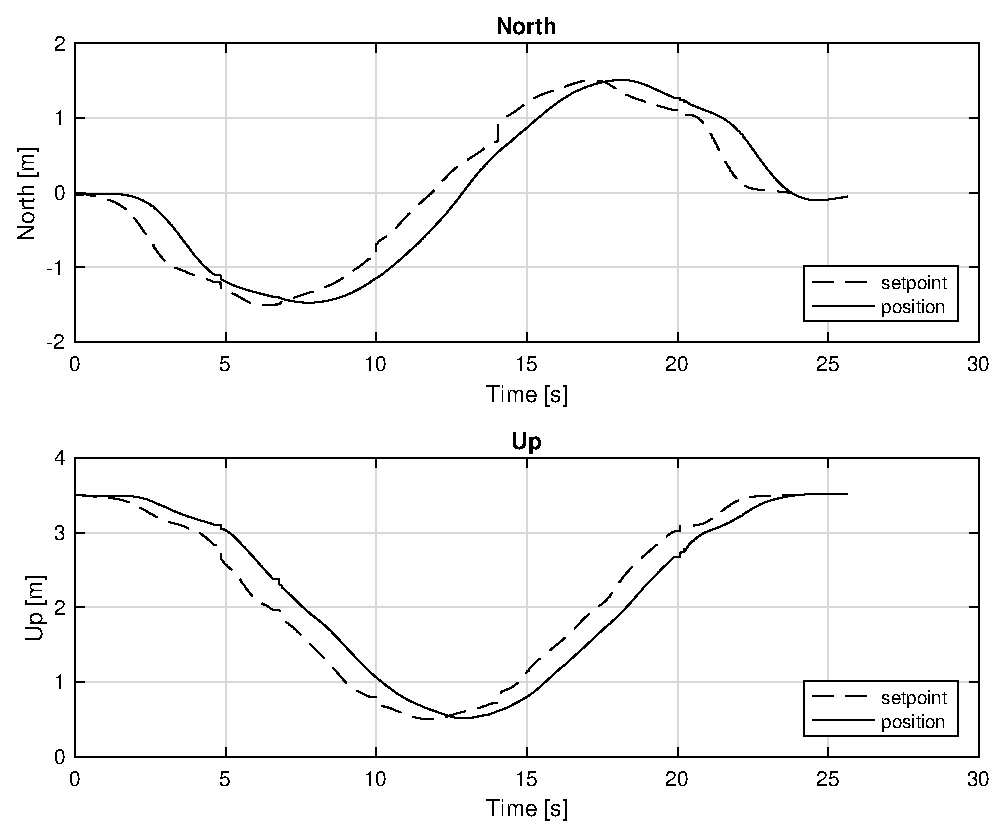
\includegraphics[width=0.7\linewidth]{chapters/chapter-05/figures/following_1.eps}
\caption{Target following drone 1}
\label{fig:exp_following_1}
\end{figure}

\begin{figure}
\centering
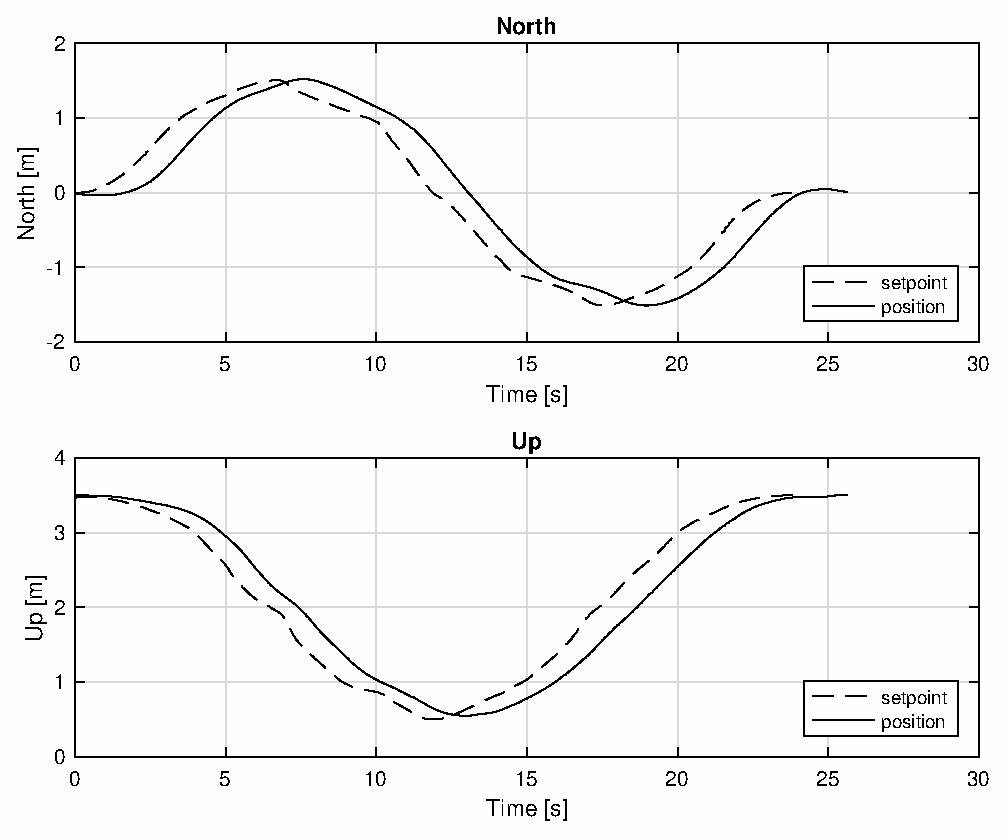
\includegraphics[width=0.7\linewidth]{chapters/chapter-05/figures/following_2.eps}
\caption{Target following drone 2}
\label{fig:exp_following_2}
\end{figure}

Even in this case, there are some delays due to the time needed to the autopilot to follow
the target, but the drones are capable of doing that.
The two drones stay synchronized during all the mission as we can see in the Figure
\ref{fig:exp_overlapped}.

\begin{figure}
\centering
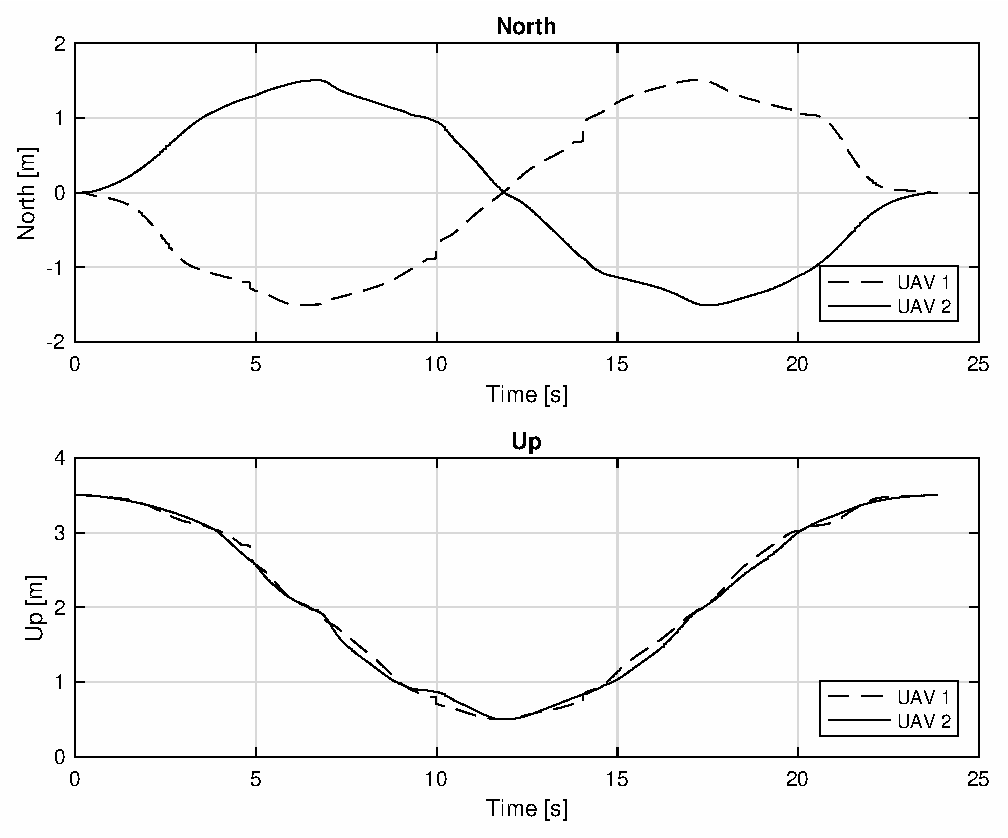
\includegraphics[width=0.7\textwidth]{chapters/chapter-05/figures/overlapped.eps}
\caption{Two drones positions over time}
\label{fig:exp_overlapped}
\end{figure}


\section{First disturbance}

When we add a disturbance to one of the drones, the algorithm rejects it and preserves
the formation. In this experiment we introduce the disturbance a time 6s and it
terminates after 10s. We see the mission in the Figures \ref{fig:exp_following_1_1}
and \ref{fig:exp_following_2_1}.

\begin{figure}
\centering
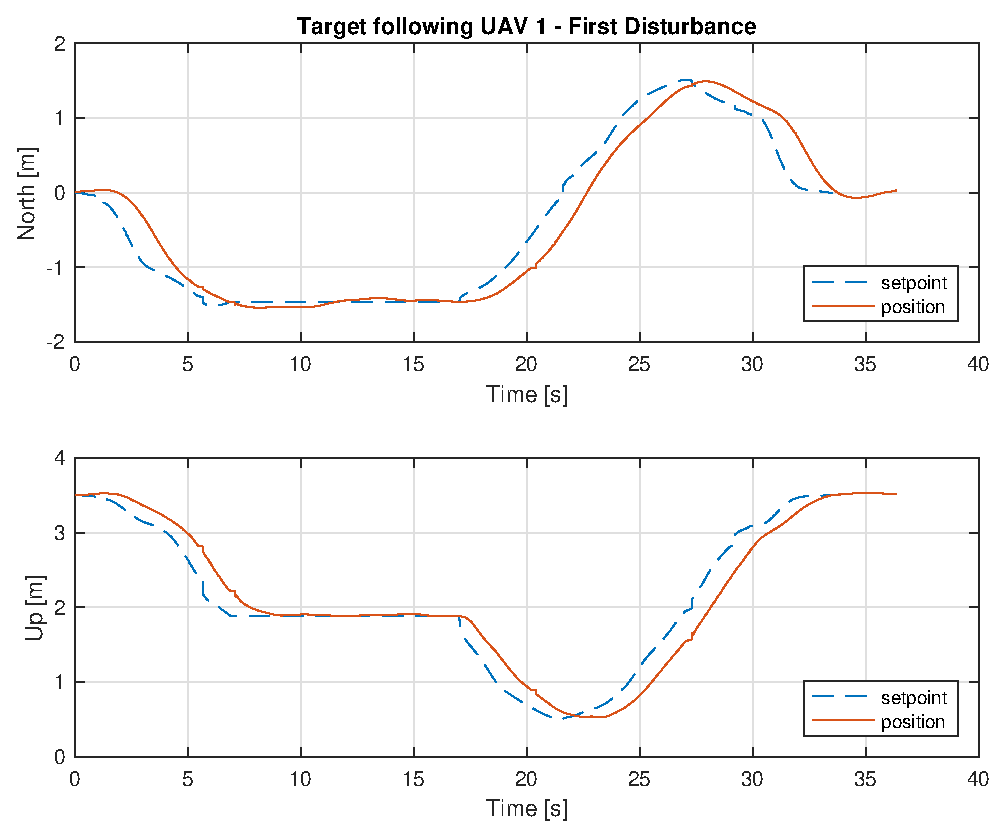
\includegraphics[width=0.7\linewidth]{chapters/chapter-05/figures/following_1_1.eps}
\caption{Target following drone 1}
\label{fig:exp_following_1_1}
\end{figure}

\begin{figure}
\centering
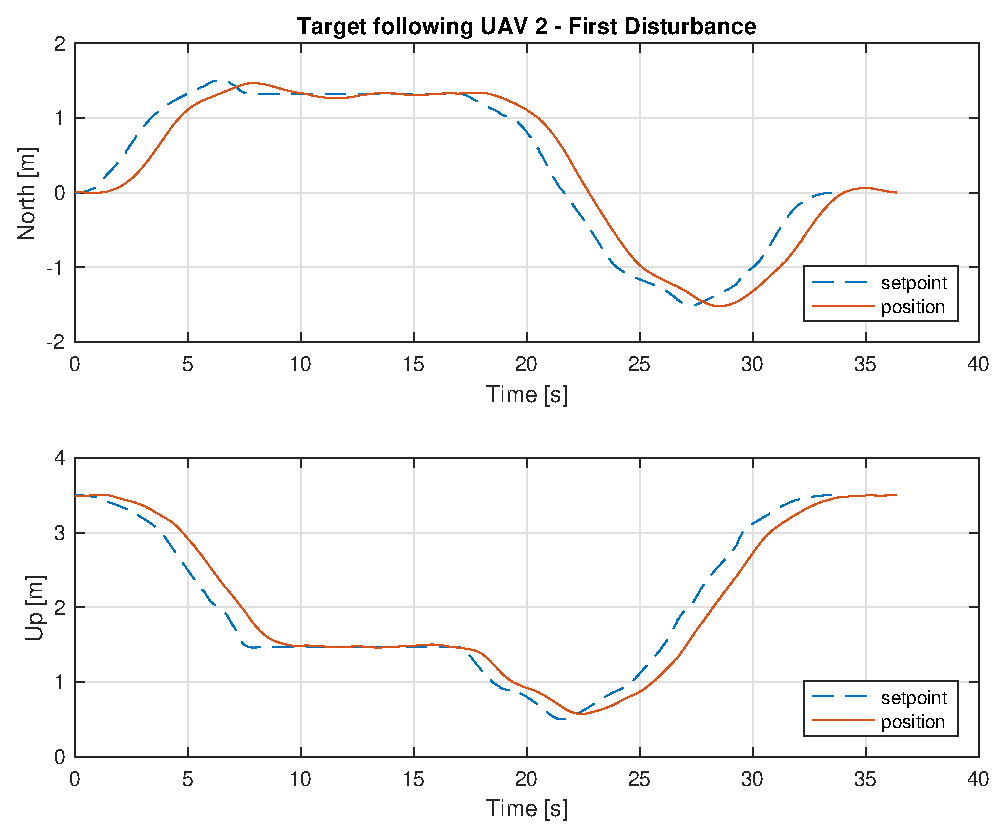
\includegraphics[width=0.7\linewidth]{chapters/chapter-05/figures/following_2_1.eps}
\caption{Target following drone 2}
\label{fig:exp_following_2_1}
\end{figure}

The disturbance causes the other drone to stop and wait until the disturbance
is finished. We can see the synchronization in the Figure \ref{fig:exp_overlapped_1}.

\begin{figure}
\centering
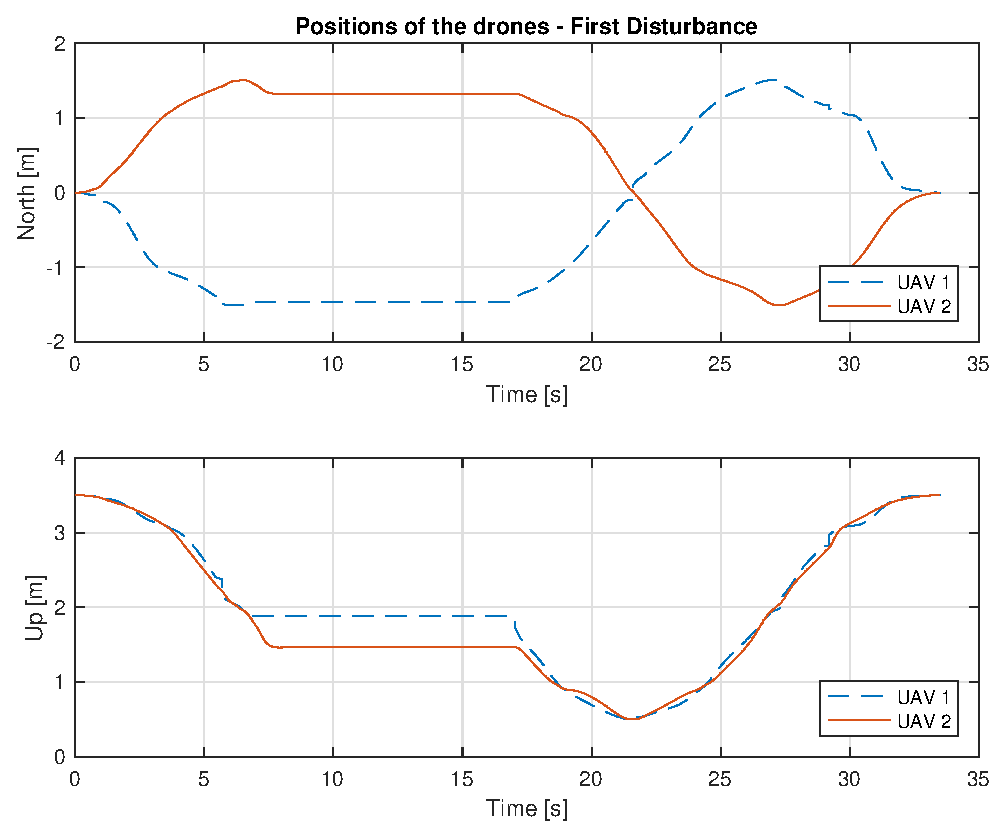
\includegraphics[width=0.7\textwidth]{chapters/chapter-05/figures/overlapped_1.eps}
\caption{Two drones positions over time}
\label{fig:exp_overlapped_1}
\end{figure}

\section{Second disturbance}
The last disturbance we show is the one which forces a drone to go back through the
trajectory. We can see how the setpoints are changed when the disturbance is active
and how the drones follow them. The Figures \ref{fig:exp_following_1_2}
and \ref{fig:exp_following_2_2} present the results.

\begin{figure}
\centering
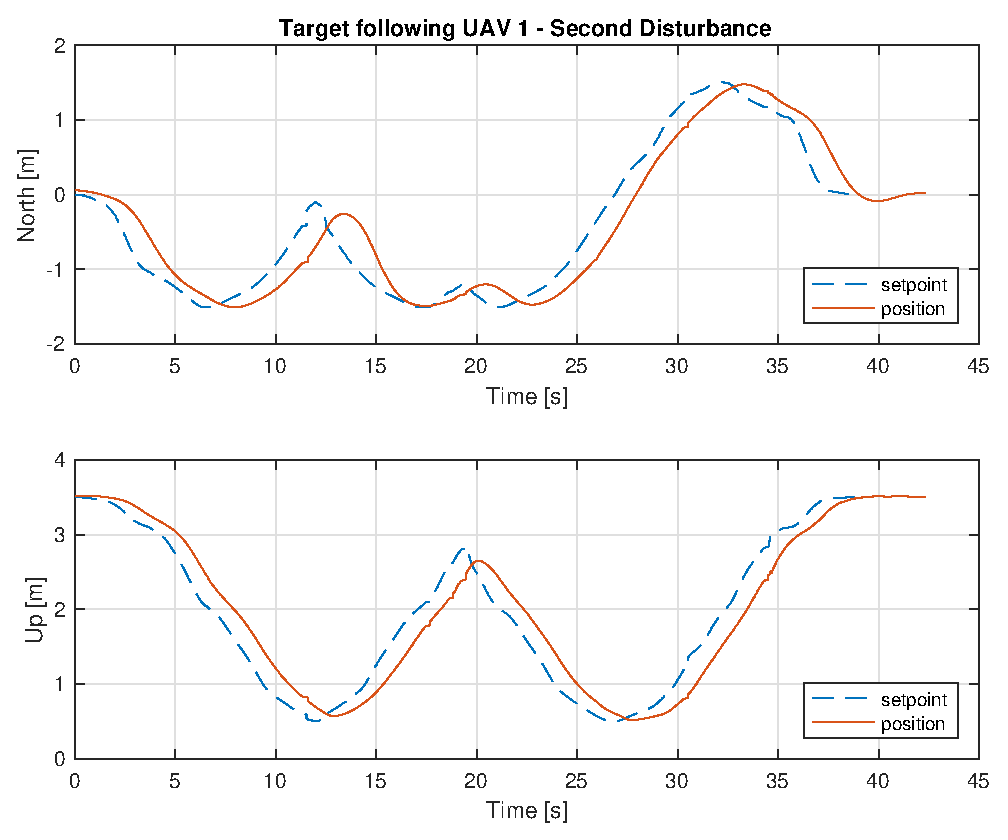
\includegraphics[width=0.7\linewidth]{chapters/chapter-05/figures/following_1_2.eps}
\caption{Target following drone 1}
\label{fig:exp_following_1_2}
\end{figure}

\begin{figure}
\centering
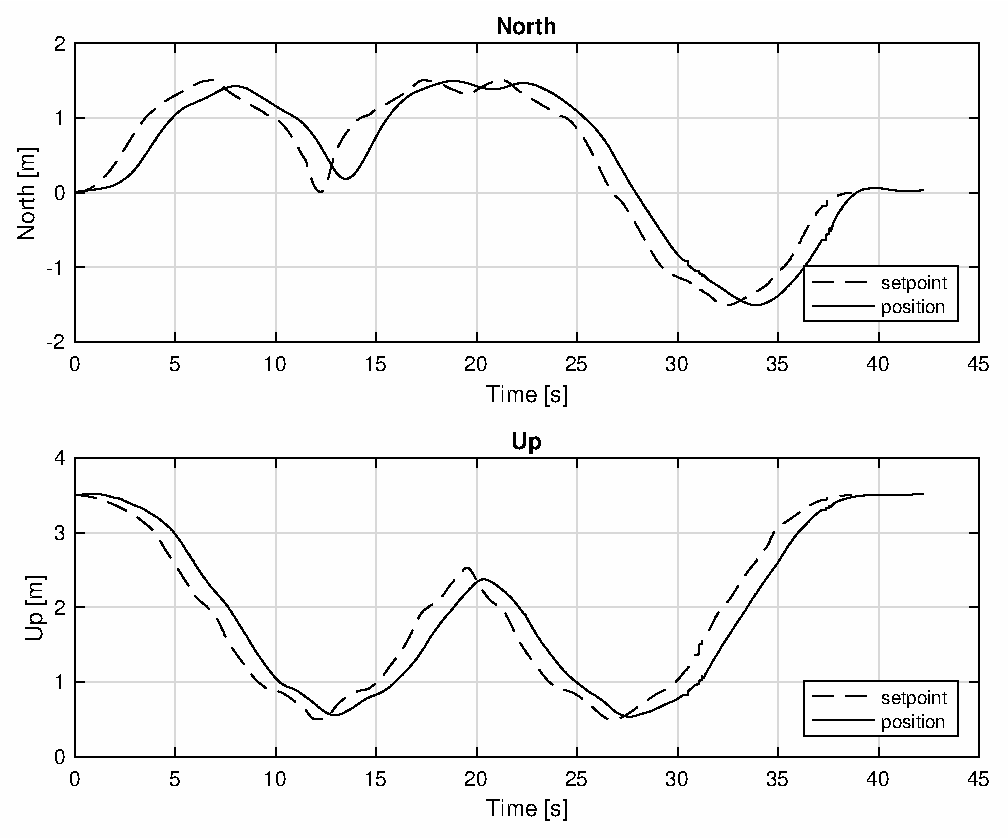
\includegraphics[width=0.7\linewidth]{chapters/chapter-05/figures/following_2_2.eps}
\caption{Target following drone 2}
\label{fig:exp_following_2_2}
\end{figure}

The disturbance causes the other drone to stop and go back, following the other,
until the disturbance is finished.
We can see the synchronization in the Figure \ref{fig:exp_overlapped_2}.

\begin{figure}
\centering
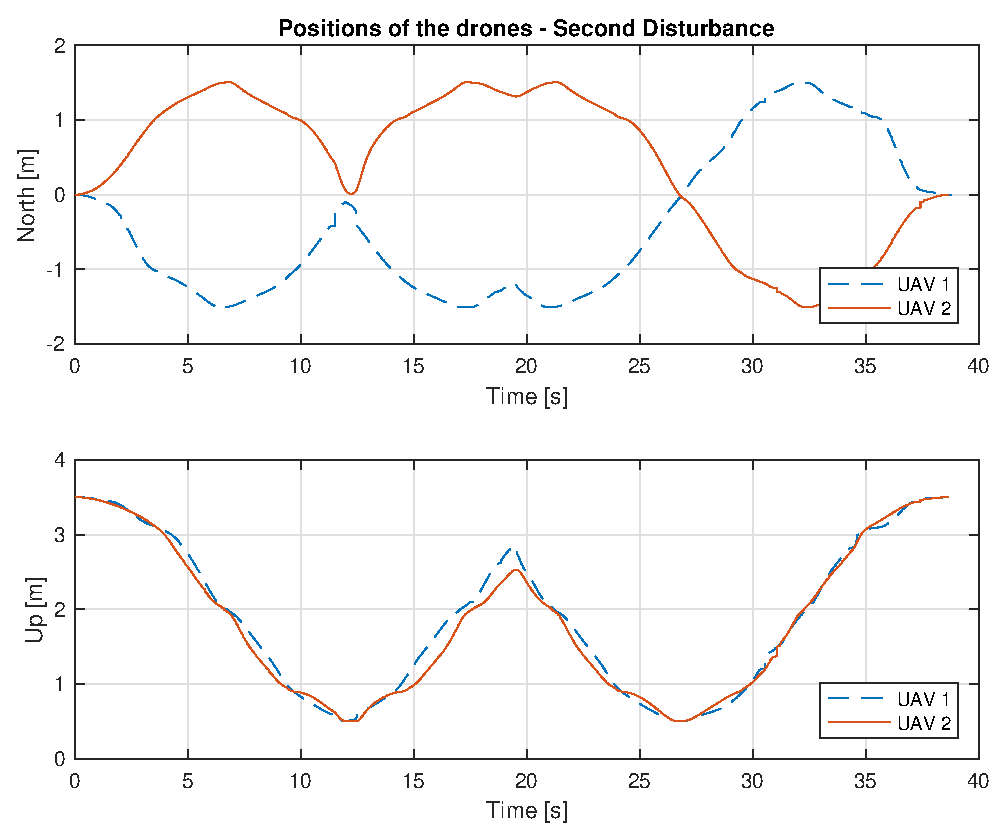
\includegraphics[width=0.7\textwidth]{chapters/chapter-05/figures/overlapped_2.eps}
\caption{Two drones positions over time}
\label{fig:exp_overlapped_2}
\end{figure}

The experimental results are less accurate than the simulated ones,
but the overall behaviour is preserved. Indeed, if we compare the results, we
can see that the formation is maintained in both cases. The plots are very similar
even if the simulated model of the drones does not reflect the real drones and even if
the drones used are heterogeneous.
